\chapter{Related Work}
  The following four approaches are all solutions that are graph-based and target a centralized and static channel assignment.
  Those are not the only ones on this matter, but the approaches currently in use and most relevant contestants to solve our problem.
  Note that there are also numerous solutions on distributed and/or dynamic or semi-dynamic environments, which we will not cover here (See Chapter \ref{reqana}).
  Except the \ac{BFS-CA}, the prevalent solutions make excessive use of the conflict graph, which according to Si et al. \cite{overview_caa} has difficulties to model 
  the varying number of radios equipped on APs. 
  Also, most of the works solely focus on assigning channels to an existing topology and do not touch the network topology at all,
  what seems like a handicap as topology control is an essential part in dealing with wireless interference as we will see later.
  
  \begin{figure}[h!]
    \centering
    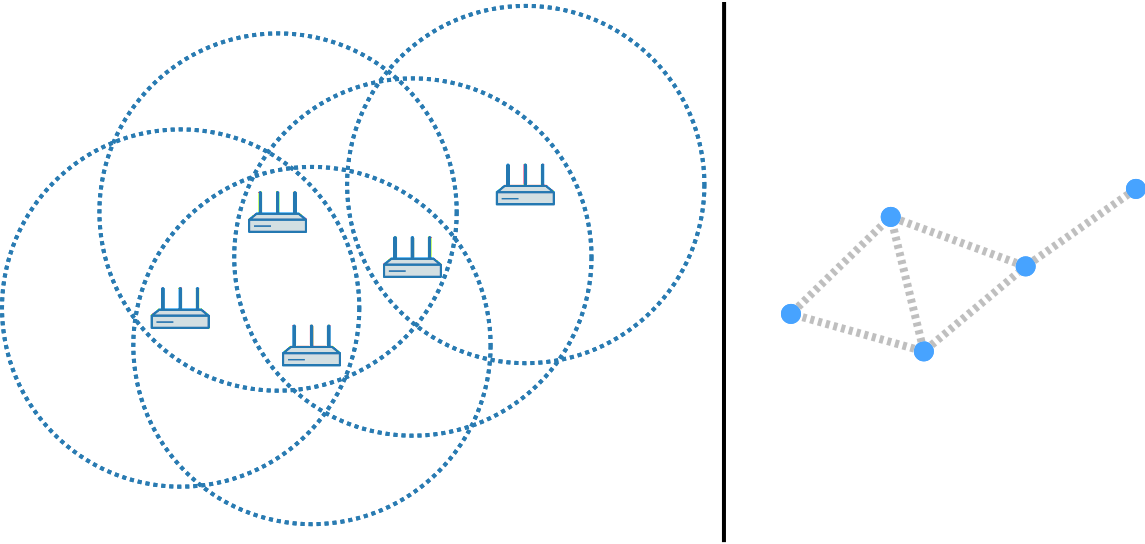
\includegraphics[width=1\columnwidth]{figures/unit-disk-graph}
    \caption{Creation of an unit disk graph from the receive range map of APs}
    \label{fig:unit-disk-graph}
  \end{figure}
  
  \section{\ac{CLICA}}
    The aim of \ac{CLICA} \cite{CLICA} is to minimize interference conflicts for a given unit disk graph preserving the connectivity.
    That means it takes the given network topology-graph as granted and tries to minimize the overall interference by resolving conflicts as much as possible.
    It takes the following parameters as input:
    
    \begin{itemize}
      \item Unit disk graph
      
      \item Number of radios at each node and total number of channels available
      
      \item Interference conflicts in form of a conflict graph
    \end{itemize}
    
    CLICA's mode of operation is described by Si et al. \cite{overview_caa} as follows:
    \begin{itemize}
      \item Randomly assign a node \(v\) the highest priority, then assign other nodes priorities decreasing in the order obtained by depth.
	
      \item While traversing the nodes in the decreasing order of their priorities obtained above, assign channels to the incident links of these nodes. 
	The operation of assigning a channel to a link includes assigning this channel to both, a radio at this node and a radio at the neighbor node. 
	Then, the priorities of unvisited nodes are adjusted according to their degree of flexibility,
	which is the number of channels that a node can choose from without breaking the connectivity preservation.
	Essentially, the nodes 	with a lower degree of flexibility will have their priorities increased so that they are visited earlier in the later steps.
	
      \item When picking a channel in the above step, a node \(v_1\) picks a channel for its incident link (\(v_1\), \(v_2\)) in a greedy manner:
	A locally optimal choice is made by selecting the channel that minimizes the maximum link-conflict-weight among all links that can interfere with link (\(v_1\), \(v_2\)).
	After a channel is assigned to a link the conflict graph is updated to reflect the new link conflict weights.
    \end{itemize}
  
    The reason why we decided not to use this algorithm is that \ac{CLICA} only tries to minimize interference by assigning channels the best way possible for a given
    unit disk graph, which is basically each possible connection.
    For a highly connected network topology like in Figure \ref{fig:graphseen} this would lead to suboptimal results
    as it does not restrict itself to necessary connections and therefore possesses a lot of potential for interference.
    The restriction to use only the best and absolutely necessary links is a vital part in order to further decrease interference as much as possible for such a topology.
    
\newpage
    
  \section{\ac{INSTC}}
    As pointed out by Si et al. \cite{overview_caa}, \ac{INSTC} \cite{INSTC} is similar to \ac{CLICA} \cite{CLICA} with a some alterations, 
    which is why we will not go into further detail and rather focus on its differences. 
    They introduce \ac{LCI}, which for a link represents the number of links which interfere with this link and serves as a measure of interference.
    Additionally, they accept \(k\) as an input parameter which results in a \(k\)-connected graph as outcome to make the topology resilient to node failures.
    Although this feature would come in handy for our survival path requirement,
    it does not match our failing scenario of a single link at a time instead of a whole node outage.
    Using a \textit{k}-(node)-connected graph instead of an \textit{k}-edge-connected graph increases the number of edges that have to be utilized 
    (since one failing node involves multiple failing edges).
    Consequently the resulting network topology has a higher grade of connectivity than it needs to 
    have and therefore conversely affects overall throughput since a higher node connectivity leads to fewer usable different channels. 
    Additional to the weaknesses of \ac{CLICA}, they also require the number of radio modules to be identical on each \ac{AP}, 
    which is a deal-breaker for us as we have to be able to fulfill requirement \ref{utilvarnumradio} (Utilize Variable Number of Radios).
    The \ac{LCI} measure introduced here served as a basis for our edgescore calculation in Formula \ref{eq:edgescore}.
    
  \section{\ac{BFS-CA}}
    \ac{BFS-CA} \cite{BFS-CA} extends the common conflict graph with modules, resulting in a \ac{MCG}, which more closely reassembles the real world setup.
    This makes it easier for them to deal with the different numbers of radios available on each device. 
    They let the APs (or mesh routers in their case) sniff the network on regular intervals and determine a ranking for the channels.
    Those rankings are then sent to their central entity, the \ac{CAS}.
    This \ac{CAS} in turn derives the \ac{MCG} and assigns each node in this graph a channel in \ac{BFS}-manner by considering the received rankings of the APs.
    In order not to partition the network by introducing a \ac{CA}, which would disconnect some links by setting certain radios to different channels,
    they also use one radio on each AP on an overall-common channel.
    This common channel is then used for initial setup, management frames and as a backup if other links break in order to keep the graph connectivity attribute.
    
    Although \ac{BFS-CA}, as others, is still anxious about topology alterations, since at a first glance it might introduce too severe problems like, 
    additional hops for packets, increased interference footprint and higher susceptibility to errors due to longer travel times of packets.
    Nevertheless it is the algorithm which we were inspired by the most and therefore have some ideas in common.
    The interesting features we reused and refined are:
    
    \begin{itemize}
     \item Idea of a ranking system for each possible channel
     
     \item Central computation on a \ac{CAS}, which reassembles our \ac{WLC}.
     
     \item Taking foreign sources of interference into consideration as well.
     
    \end{itemize}
    
\newpage
    
    Yet, we decided against its implementation for our purposes for the following reasons:
    
    \begin{itemize}
      \item Using all possible channels in the network topology creates to much interference for networks with more traffic.
	A selection process on this underlying topology is essential to our minds as selecting a few but high quality links
	leading to a planned and controlled topology will create a lot less interference than a network topology where all possible 	links are used for communications.
	This is especially the case if not enough channels are available for assignment,
	since these can be more effectively designed (See Chapter \ref{fig:high_con_vs_low_con}).
	\label{topologypreservingdealbreaker}
	
      \item Using one radio on each \ac{AP} for a common overall-channel seemed to us as a misspending of radio modules.
	Radio modules on APs are scarce and should be utilized efficiently. 
	Furthermore one overall-channel which is utilized by each \ac{AP} does not scale well and is basically already done in \textit{AutoWDS basic}.
	
      \item The ranking process, suggested to run on the APs, creates load on the APs.
	We want to use the APs merely as sensors and not as decision-makers, 
	since this puts additional load on the APs and brings problems/complexity with synchronisation and acquiring the overall view on the network.
	
      \item The ranking algorithm itself could be improved. 
	The solution averages values too early in the process and uses a random pick not as a last resort - providing supoptimal results.
	
      \item \ac{BFS}'s order of assigning channels puts one node (gateway-node) above all others during channel assignment.
	In some of our use cases there is no gateway-node available (See Section \ref{reqincreasethroughput}) and we need a fair distribution of channels, 
	which is not feasible with this solution \cite{overview_caa}.
    \end{itemize}

  \section{\ac{CTA}}
    Subramanian et al. \cite{CTA} use a modified Tabu-algorithm \cite{tabu} in two steps to find a \ac{CA} for the conflict graph.
    It works by starting with a random \ac{CA} and, like an evolutionary algorithm, 
    iteratively changing small details and selecting the best temporal solution to continue for the next iteration.
    An iteration is here further subdivided into generating a number of random neighboring assignments,
    where only the color / channel of one vertex is changed.
    From this set they select the assignment with the lowest interference.
    The tabu-list, which describes the forbidden options which are not allowed to be chosen for improvement,
    contains a list of vertex-colorings that already have been used.
    This procedure is then executed as long as there have been improvements in the last \textit{$i_{max}$} rounds.
    If for \textit{$i_{max}$} rounds no improvement can be found, the algorithm proceeds with step two.
    As the first step may give channel assignings which are not valid (more channels assigned than a node has radios), 
    the second step merges channel assignments until the solution is valid again.
    Merging channels obviously increases the interference.
    
    This solution is also topology preserving and a deal-breaker for our implementation (See Section \ref{topologypreservingdealbreaker}).
    Additionally the evolutionary attribute does not provide controlled, but more heuristic results and we need an algorithm with more control over its internals.